% Created 2018-11-13 Tue 22:06
% Intended LaTeX compiler: pdflatex
\documentclass[presentation]{beamer}
\usepackage[utf8]{inputenc}
\usepackage[T1]{fontenc}
\usepackage{graphicx}
\usepackage{grffile}
\usepackage{longtable}
\usepackage{wrapfig}
\usepackage{rotating}
\usepackage[normalem]{ulem}
\usepackage{amsmath}
\usepackage{textcomp}
\usepackage{amssymb}
\usepackage{capt-of}
\usepackage{natbib}
\usepackage[linktocpage,pdfstartview=FitH,colorlinks,
linkcolor=blue,anchorcolor=blue,
citecolor=blue,filecolor=blue,menucolor=blue,urlcolor=blue]{hyperref}
\setbeamertemplate{frame footer}{\insertshortauthor}
\setbeamerfont{page number in head/foot}{size=\tiny}
\setbeamercolor{footline}{fg=gray}
\usepackage{amsmath}
\author{Florian Hollenbach}
\usepackage[english]{isodate}
\usepackage{amsmath,amsthm,amssymb,amsfonts}
\newcommand{\E}{\mathbb{E}}
\newcommand{\V}{\mathbb{V}}
\usetheme{metropolis}
\usecolortheme{}
\usefonttheme{}
\useinnertheme{}
\useoutertheme{}
\author{Florian Hollenbach}
\date{\today}
\title{Political Science 209 - Fall 2018}
\subtitle{Uncertainty}

\hypersetup{
 pdfauthor={Florian Hollenbach},
 pdftitle={Political Science 209 - Fall 2018},
 pdfkeywords={},
 pdfsubject={},
 pdfcreator={Emacs 25.3.1 (Org mode 9.1.14)}, 
 pdflang={English}}
\begin{document}

\maketitle


\begin{frame}[label={sec:orgdc272e1}]{Statistical Inference}
Goal: trying to estimate something unobservable from observable data

What we want to estimate: \alert{parameter} \(\theta\) \(\rightsquigarrow\) unobservable

What you do observe: \alert{data}

\pause

We use data to compute an estimate of the parameter \(\hat\theta\)
\end{frame}


\begin{frame}[label={sec:orgd2edaba}]{Parameters and Estimators}
\begin{itemize}
\item \alert{parameter}: the quantity that we are interested in
\end{itemize}

\pause

\begin{itemize}
\item \alert{estimator}: method to compute parameter of interest
\end{itemize}
\end{frame}

\begin{frame}[label={sec:org9e882ec}]{Parameters and Estimators}
Example:

\begin{itemize}
\item \alert{parameter}: support for Jimbo Fisher in student population

\item \alert{estimator}: sample proportion of support as estimator
\end{itemize}
\end{frame}

\begin{frame}[label={sec:org82dcac4}]{Parameters and Estimators}
Example:

\begin{itemize}
\item \alert{parameter}: average causal effect of aspirin on headache

\item \alert{estimator}: difference in mean between treatment and control
\end{itemize}
\end{frame}


\begin{frame}[label={sec:orgdaf3354}]{Quality of estimators}
For the rest of the semester the question becomes:

\alert{How good is our estimator?}

\pause

\begin{enumerate}
\item \alert{How close in expectation is the estimator to the truth?}

\item \alert{How certain or uncertain are we about the estimate?}
\end{enumerate}
\end{frame}

\begin{frame}[label={sec:orga142d5b}]{Quality of estimators}
How good is \(\hat\theta\) as an estimate of \(\theta\)?

\begin{itemize}
\item Ideally, we want to know \alert{estimation error} \(= \hat\theta - \theta_{truth}\)
\end{itemize}

But we can never calculate this. Why?

\pause

\(\theta_{truth}\) is unknown

\emph{If we knew what the truth was, we didn't need an estimate}
\end{frame}

\begin{frame}[label={sec:orge68735c}]{Quality of estimators}
Instead, we consider two hypothetical scenarios:
\begin{enumerate}
\item How well would \(\hat\theta\) perform over \emph{repeated data generating processes}? (\alert{bias})
\item How well would \(\hat\theta\) perform as the sample size goes to infinity? (\alert{consistency})
\end{enumerate}
\end{frame}

\begin{frame}[label={sec:org5952200}]{Bias}
\begin{itemize}
\item Imagine the estimate being a random variable itself

\item Drawing infinitely many samples of students asking about Jimbo
\end{itemize}

What is the average of the sample average? Or what is the expectation of the estimator?

bias = \(\E\)(estimation error) = \(\E\)(estimate - truth) = \(\E(\bar{X})\) - p = p - p = 0
\end{frame}


\begin{frame}[label={sec:orgfb944bc}]{Bias - \alert{Important}}
\alert{An unbiased estimator does not mean that it is always exactly correct!}

\pause
\alert{To remember:} bias measures whether in expectation (on average) the estimator is giving us the truth
\end{frame}

\begin{frame}[label={sec:orgb9f7716}]{Consistency}
Essentially saying that the law of large numbers applies to the estimator, i.e.:

\alert{An estimator is said to be consistent if it converges to the parameter (truth) if N goes to \(\infty\)}
\end{frame}


\begin{frame}[label={sec:org146117a}]{Variability}
Next, we have to consider how certain we are about our results

Consider two estimators:

\begin{enumerate}
\item slightly \emph{biased}, on average off by a bit, but always by the same margin

\item unbiased, but misses target left and right
\end{enumerate}
\end{frame}


\begin{frame}[label={sec:orgfca3e86}]{Variability}
\begin{center}
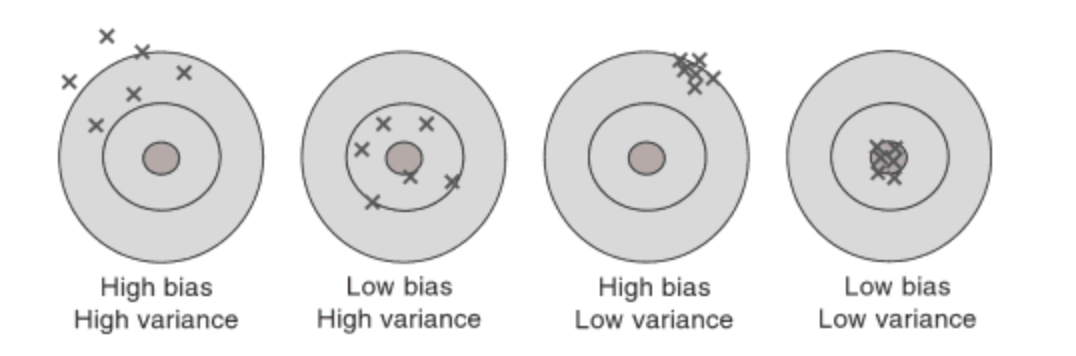
\includegraphics[width=6cm]{/Users/florianhollenbach/Documents/GitHub/Polisci209_2018/slides/week13/DART.png}
\end{center}

(Encyclopedia of Machine Learning)
\end{frame}

\begin{frame}[label={sec:org77c446c}]{Variability}
We characterize the variability of an estimator by using the standard deviation of the sampling distribution

\alert{How do we find that????}

\pause

Remember, the sampling distribution is the distribution of our statistic over hypothetical infinitely many samples
\end{frame}

\begin{frame}[label={sec:org7324b6e}]{Variability}
\begin{center}
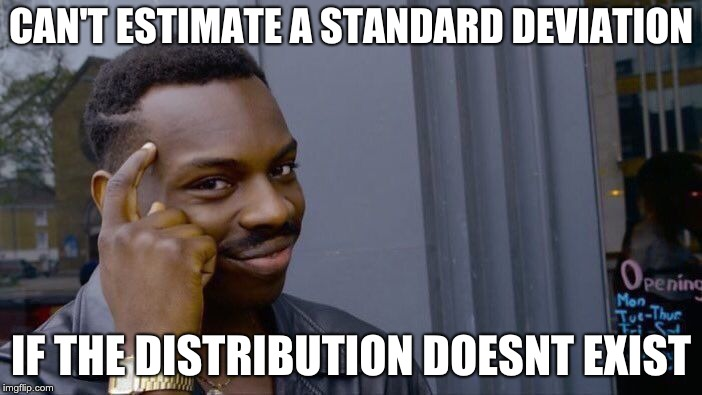
\includegraphics[width=6cm]{/Users/florianhollenbach/Documents/GitHub/Polisci209_2018/slides/week13/2mi1j5.jpg}
\end{center}
\end{frame}


\begin{frame}[label={sec:orgc195972}]{Standard Error}
We estimate the standard deviation of the sampling distribution from the observed data

\alert{standard error}

\pause

``\emph{standard error} and describes the (estimated) average degree to which an estimator deviates from its expected value'' (Imai 2017)
\end{frame}

\begin{frame}[label={sec:org729996d}]{Polling Example}
Say we took a sample of 1000 students and asked whether they support Jimbo or not

Define a random variable \(X_{i} = 1\) if student \emph{i} supports Jimbo, \(X_{i}=0\) if not

Binomial distribution with success probability p and size N where p is the proportion of \emph{all students} who support Jimbo (population dist)
\end{frame}


\begin{frame}[label={sec:orgca5dc6b}]{Polling Example}
Estimator: ?
\end{frame}

\begin{frame}[label={sec:org67f2b2b}]{Polling Example}
Estimator: \(\overline{X} = \frac{1}{N} \sum_{i=1}^{N} X_{i}\)

\pause

In earlier notation: \(\theta_{truth} =p\) and \(\theta = \overline{X}\)
\end{frame}


\begin{frame}[label={sec:org55bb2fa}]{Polling Example}
Estimator: \(\overline{X} = \frac{1}{N} \sum_{i=1}^{N} X_{i}\)

\begin{enumerate}
\item LLN: \(\overline{X} \longrightarrow p\) (\alert{consistent})

\item Expectation: \(\E(\overline{X}) = p\) (\alert{unbiased})

\item standard error?
\end{enumerate}
\end{frame}


\begin{frame}[label={sec:org57d9614}]{Polling Example - standard error}
\(X_i\) are i.i.d Bernoulli random variables with probability = p


\(\V(\overline{X}) = \frac{1}{N^{2}} \V(\sum_{i=1}^{N}X_{i})  = \frac{1}{N^{2}} \sum_{i=1}^{N} \V(X_{i})\)
\end{frame}


\begin{frame}[label={sec:orga70202d}]{Polling Example - standard error}
\(X_i\) are i.i.d Bernoulli random variables with probability = p


\(\V(\overline{X}) = \frac{1}{N^{2}} \V(\sum_{i=1}^{N}X_{i})  = \frac{1}{N^{2}} \sum_{i=1}^{N} \V(X_{i}) = \frac{N}{N^{2}} \V(X)\)
\end{frame}


\begin{frame}[label={sec:org48ddebd}]{Polling Example - standard error}
\(X_i\) are i.i.d Bernoulli random variables with probability = p


\(\V(\overline{X}) = \frac{1}{N^{2}} \V(\sum_{i=1}^{N}X_{i})  = \frac{1}{N^{2}} \sum_{i=1}^{N} \V(X_{i}) = \frac{N}{N^{2}} \V(X) = \frac{p \times (1-p)}{N}\)
\end{frame}

\begin{frame}[label={sec:org064ee51}]{Polling Example - standard error}
\(\V(\overline{X}) = \frac{p \times (1-p)}{N}\)

Standard error: \(\sqrt{\V(\overline{X})}\)

But we don't know p! Now what?

\pause

We use our unbiased estimate of p: \overline{X}
\end{frame}

\begin{frame}[label={sec:org687bc0d}]{Polling Example - standard error estimate}
\(\sqrt{\widehat{\V(\overline{X})}} = \sqrt{\frac{\overline{X}(1-\overline{X})}{N}}\)
\end{frame}

\begin{frame}[label={sec:orgcaabb41}]{Polling Example - standard error estimate}
Assume in our sample 55\% of students support Jimbo:

SE = \(\sqrt{\widehat{\V(\overline{X})}} = \sqrt{\frac{0.55 \times (1-0.55)}{1500}} = \sqrt{\frac{0.55 \times (0.45)}{1000}} = 0.016\)

We can expect our estimate on average to be off by 1.6 percentage points

\pause

If \(\overline{X}\) = 0.8, then SE = 0.012

If N = 500, \(\overline{X}\) = 0.55, then SE = 0.022
\end{frame}

\begin{frame}[label={sec:org6cb1772}]{Standard error estimate}
Standard error is based on variance of the sampling distribution

Gives estimate of uncertainty

Each estimator/statistic has unique sampling distribution, e.g. difference in means
\end{frame}

\begin{frame}[label={sec:org52c443e}]{Confidence Intervals}
\end{frame}
\end{document}